\documentclass[a4paper,10pt]{article}
\usepackage[utf8]{inputenc}
\usepackage{amsmath, amsfonts, graphicx}
\usepackage{hyperref}
\usepackage{indentfirst}
%opening
\title{}
\author{}

\begin{document}


\section{Manifold}

In this post I would like to speak about an abstract mathematical construction called {\it manifold}. In the future we will work with a limited number of manifolds, however, I believe that introducing some fundamental concepts of the theory of manifolds is, at least, useful. 

Let us call a {\it topological space } a set of points where there are defined all open subsets. We will not go any deeper into this definition. For more information about the topological spaces like what is an {\it open subset} check the wikipedia article \cite{topspace}. 

On the other hand, we are not interested in the most general topological spaces rather those on which we can define {\it coordinate systems}. We are familiar with the Euclidean space. See Figure \ref{fig:3dcart}

\begin{figure}[h]
\centering
 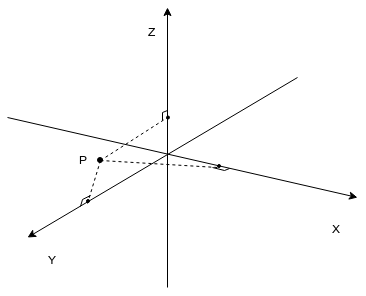
\includegraphics[width=0.6\textwidth]{../../images/3DEuclidean.png}
 \caption{The 3-dimensional Euclidean space with Cartesian coordinate axis. The 3 coordinates $(x,y,z)$ are determined by passing perpendiculars to the corresponding axis and measuring the distance between the intersection points and the origin. }
 \label{fig:3dcart}
\end{figure}
 
To any point in the Euclidean space $\mathbb{R}^n$  we can uniquely assign a set of Cartesian coordinates $(x_1, x_2,\ldots, x_n)$. Conversely, the set of Cartesian coordinates $(x_1, x_2,\ldots, x_n)$ uniquely determines a point in the Euclidean space. 

We know, how to introduce the coordinate systems in $\mathbb{R}^n$. Let us see how we can utilize it for defining a coordinate system on a generic topological space $M$. Assume we can define a continuous (maps open subsets to open subsets) invertable map $\varphi$ from an open subset $U$ of $\mathbb{R}^n$ onto an open subset of $M$. By doing so, we automatically cover that subset with a coordinate system. Indeed, for any set of coordinates $(x_1, x_2,\ldots, x_n)$ we will have a unique point in $\mathbb{R}^n$, which in its turn corresponds to a unique point on the subset $\varphi U \subset M$ via the map $\varphi$ (Fig \ref{fig:phimap}). 

\begin{figure}[h]
\centering
 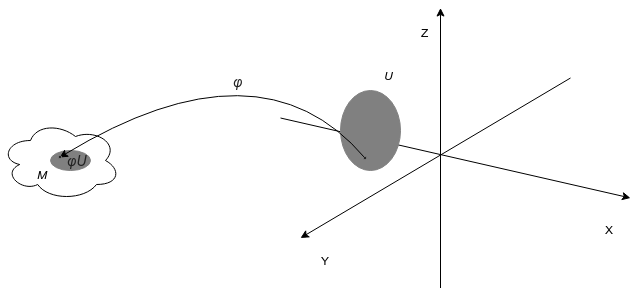
\includegraphics[width=0.6\textwidth]{../../images/PhiMap.png}
 \caption{Mapping from an open subset of 3D Euclidean space onto an open subset of $M$}
 \label{fig:phimap}
\end{figure}

This map, together with the open subset $U\subset \mathbb{R}^n$ is called a {\it chart} on $M$. If it is possible to cover the entire $M$ with a finite or countable number of such charts so that any point on $M$ will be covered by at least one of them, then we will have coordinate system on the entire $M$. In order to specify a point on $M$ one has to specify the chart $(\varphi^i, U^{(i)})$ and a set of coordinates $(x_1^{(i)}, \ldots, x_n^{(i)})\in U^{(i)}$. 

The set of the charts is called {\it atlas}. A topological space with an {\it atlas} is called {\it manifold}. 
In other words, a {\it manifold} is a topological space, which { \it locally } (in a neighborhood of a point) looks like a Euclidean space. 

If some point of $M$ is on two charts $U$ and $U'$ then there are some neighborhoods $V$ and $V'$ of that point on each of the charts such that all points in that neighborhoods are pictured on both charts. Hence, we have a natural mapping $\phi'^{-1}\phi: V\mapsto V'$ of a part $V\subset U$ of one chart on a part of the other $V'\subset U'$ \cite{arn, egh}.

Let us consider a few examples.

\section{Examples}


{\bf Euclidean space $\mathbb{R}^n$}
\newline

Obviously, the Euclidean space is a manifold by itself. 
\newline

{\bf Sphere $S^2$}
\newline

A unit sphere in 3D-space is defined by the following constraint:

\begin{equation}
 x^2 + y^2 + z^2 = 1
\end{equation}

Obviously, the sphere is a 2-dimensional manifold. To define a chart on the sphere, consider a 2D-plane $\mathbb{R}^2$ with its Cartesian coordinate system which $x$ and $y$ axis coincide with $X$ and $Y$ respectively. Let us connect the point $P'$ on $(x,y)$ plane to the North Pole with a line. The corresponding point $P$ on the sphere would be the point of the intersection of that line with the sphere.  Figure \ref{fig:riemann}.

\begin{figure}[h]
\centering
 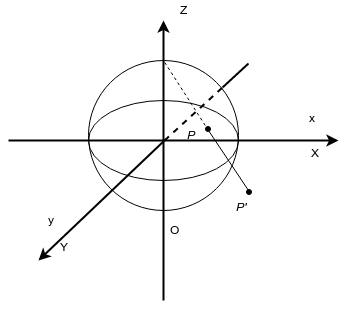
\includegraphics[width=0.7\textwidth]{../../images/Sphere.png}
 \caption{The projective coordinates on 2D-sphere.  }
 \label{fig:riemann}
\end{figure}

In this way, we establish a correspondence between all points on $\mathbb{R^2} \equiv U$ with all points of sphere except the North Pole itself. To cover the whole sphere with  charts we should repeat our construction using the South Pole instead. This second chart will cover the entire sphere except the South Pole. 

For completeness, let us present the mapping from $(X,Y,Z)$ coordinates of the ambient $\mathbb{R}^3$ to the chart coordinates $(x,y)$.

\begin{equation}
 x = \frac{X}{1\pm Z},\quad y = \frac{y}{1\pm Z}
\end{equation}
and the inverse 

\begin{equation}
 X = \frac{2x}{1+\rho^2},\quad Y = \frac{2y}{1+\rho^2}, \quad Z = \frac{1\mp\rho^2}{1\pm\rho^2}, 
\end{equation}
where $\rho^2 = x^2 + y^2$

A straightforward generalization of this construction exists for any dimensional sphere. Hence, all spheres are covered by two charts.
\newline

{\bf Projective space}
\newline

Real projective space $\mathbb{RP}^n$\footnote{ In contrast to complex projective space $\mathbb{CP}^n$, which is out of our consideration.  } is the set of lines in $\mathbb{R}^{n+1}$ passing through the origin. A point $x \in \mathbb{R}^{n+1}, x\neq 0$ uniquely defines a line passing through the origin. On the other hand, the same line is defined by any other point $x' = \alpha x$. 

To eliminate this arbitrariness, we can divide all coordinates by a single chosen one, thus introducing a chart on $\mathbb{RP}^n$.

\begin{equation}
\xi^{(k)}_i = \frac{x_i}{x_k},  \quad i\neq k, \quad i,k = 1, \ldots, n+1.
\end{equation}

This chart is not defined for points for which $x_k = 0$, therefore, those points are not present on it. 

For any two charts $\xi^{(j)}$ and $\xi^{(k)}$ the transition functions between them look as follows

\begin{equation}
 \xi^{(j)}_i = \frac{x_i}{x_j} \equiv \frac{x_i}{x_k}\frac{x_k}{x_j} \equiv \frac{\xi^{(k)}_i}{\xi^{(k)}_j}, \quad x_k, x_j\neq 0.
\end{equation}


\newpage
\section{Examples (non-manifolds)}

1-dimensional spaces with junctions are not manifolds.

\begin{figure}[h]
\centering
 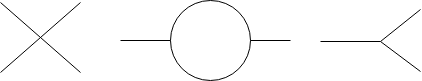
\includegraphics[width=0.7\textwidth]{../../images/NonManifolds.png}
 \caption{ 1D spaces with junctions are not manifolds.}
 \label{fig:nm}
\end{figure}

The space formed by the intersection of 2-planes is not a manifold.

\begin{thebibliography}{1}
\bibitem{topspace} \href{https://en.wikipedia.org/wiki/Topological_space}{Wiki: Topological space}
\bibitem{arn} ~V. Arnold, ``Mathematical Methods in Classical Mechanics''
\bibitem{egh} ~T., Eguchi, ~P. ~B. Gilkey, ~A. ~J. Hanson,  ``Gravitation, Gauge Theories and Differential Geometry''
\end{thebibliography}


\end{document}


